\documentclass[10pt]{beamer}
\usetheme{Madrid}
\usecolortheme{default}

\usepackage{amsmath,amssymb,amsfonts}
\usepackage{algorithm}
\usepackage{algorithmic}
\usepackage{graphicx}
\usepackage{tikz}
\usepackage{booktabs}
\usepackage{xcolor}

\title{Unpaired Neural Schrödinger Bridge (UNSB)}
\subtitle{Adversarial Learning for Unpaired Image-to-Image Translation}
\author{Research Presentation}
\date{\today}

\begin{document}

\frame{\titlepage}

\begin{frame}{Outline}
\tableofcontents
\end{frame}

\section{Motivation and Background}

\begin{frame}{The Core Problem}
\begin{block}{Central Challenge}
Learn a \alert{stochastic mapping} between two distributions $\pi_0$ and $\pi_1$ without paired data
\end{block}

\begin{columns}
\begin{column}{0.5\textwidth}
\textbf{Limitations of existing methods:}
\begin{itemize}
    \item CycleGAN: Requires cycle-consistency
    \item Diffusion models: High training cost
    \item Optimal Transport: Deterministic, lacks diversity
\end{itemize}
\end{column}

\begin{column}{0.5\textwidth}
\textbf{UNSB advantages:}
\begin{itemize}
    \item \textcolor{blue}{No paired data needed}
    \item \textcolor{blue}{Stochastic mapping}
    \item \textcolor{blue}{Theoretical guarantees}
    \item \textcolor{blue}{Efficient training}
\end{itemize}
\end{column}
\end{columns}
\end{frame}

\begin{frame}{What is Schrödinger Bridge?}
\begin{block}{Definition}
The Schrödinger Bridge (SB) seeks the \alert{optimal stochastic process} connecting two distributions that minimizes:
\begin{equation}
\min_{p(x_t)} \text{KL}(p(x_t) \| q(x_t))
\end{equation}
where $q(x_t)$ is a reference process (typically Ornstein-Uhlenbeck)
\end{block}

\begin{block}{Intuition}
SB solves a ``most likely'' stochastic interpolation problem:
\begin{itemize}
    \item Start from $\pi_0$ and end at $\pi_1$
    \item Among all stochastic processes that connect them
    \item Choose the process closest (in KL sense) to a simple reference diffusion
\end{itemize}
This yields a \textbf{stochastic and smooth} transformation unlike OT's deterministic mapping.
\end{block}

\begin{alertblock}{Key Properties}
\begin{itemize}
    \item SB is a \textbf{dynamic process}: $x_0 \sim \pi_0 \rightarrow x_t \rightarrow x_1 \sim \pi_1$
    \item Compared to OT, SB provides \textbf{stochasticity} and \textbf{smooth paths}
    \item Traditional SB requires \textcolor{red}{expensive iterative solving} (Sinkhorn iterations)
\end{itemize}
\end{alertblock}

\pause
\vspace{0.3cm}
\textbf{Question:} Why is stochasticity important in image translation?
\end{frame}

\section{Core Innovation: Markov Decomposition}

\begin{frame}{The Key Insight}
\begin{block}{Main Theorem}
UNSB represents SB as a composition of generators learned via \alert{adversarial learning}
\end{block}

\textbf{Time discretization:} Given partition $\{t_i\}_{i=0}^N$ of $[0,1]$ where $t_0=0, t_N=1$

\begin{equation}
p(\{x_{t_n}\}) = \textcolor{blue}{p(x_{t_N}|x_{t_{N-1}})} \textcolor{green!50!black}{p(x_{t_{N-1}}|x_{t_{N-2}})} \cdots \textcolor{orange}{p(x_{t_1}|x_{t_0})} p(x_{t_0})
\end{equation}

\begin{center}
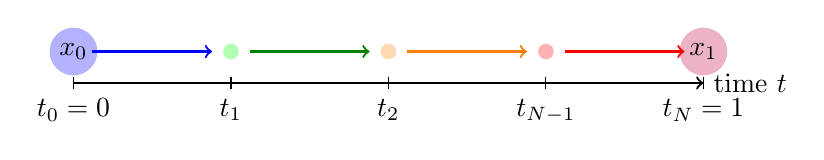
\begin{tikzpicture}[scale=0.8]
\draw[->, thick] (0,0) -- (10,0) node[right] {time $t$};
\foreach \x/\label in {0/$t_0=0$, 2.5/$t_1$, 5/$t_2$, 7.5/$t_{N-1}$, 10/$t_N=1$}
    \draw (\x,0.1) -- (\x,-0.1) node[below] {\label};
\node[circle, fill=blue!30, inner sep=2pt] at (0,0.5) {$x_0$};
\node[circle, fill=green!30, inner sep=2pt] at (2.5,0.5) {};
\node[circle, fill=orange!30, inner sep=2pt] at (5,0.5) {};
\node[circle, fill=red!30, inner sep=2pt] at (7.5,0.5) {};
\node[circle, fill=purple!30, inner sep=2pt] at (10,0.5) {$x_1$};
\draw[->, thick, blue] (0.3,0.5) -- (2.2,0.5);
\draw[->, thick, green!50!black] (2.8,0.5) -- (4.7,0.5);
\draw[->, thick, orange] (5.3,0.5) -- (7.2,0.5);
\draw[->, thick, red] (7.8,0.5) -- (9.7,0.5);
\end{tikzpicture}
\end{center}

\textbf{Inductive strategy:} Learn $p(x_{t_{i+1}}|x_{t_i})$ assuming we can sample from $p(x_{t_i})$

\begin{block}{Why this decomposition matters}
The full path distribution $p(\{x_t\}_{t\in[0,1]})$ is infinite-dimensional.
Markov factorization reduces the problem to learning only:
\[
p(x_{t_{i+1}}\mid x_{t_i}),\quad i=0,\dots,N-1,
\]
which are simple, finite-dimensional conditional distributions.
Thus UNSB avoids directly modeling the entire trajectory.
\end{block}
\end{frame}

\begin{frame}{Why Time Decomposition?}
\pause
\textbf{Challenge 1: Infinite-dimensional complexity}
\begin{itemize}
    \item Entire trajectory $\{x_t\}_{t\in[0,1]}$ is an infinite-dimensional object
    \item Direct learning: intractable path-space distribution
    \item Decomposition: learn simple conditional distributions
\end{itemize}

\pause
\vspace{0.3cm}
\textbf{Challenge 2: No intermediate data}
\begin{itemize}
    \item Only have marginals $\pi_0$ and $\pi_1$
    \item No access to trajectory samples
    \item Path density is incomputable
\end{itemize}

\pause
\vspace{0.3cm}
\textbf{Solution:} Learn $p(x_1|x_{t_i})$ (endpoint prediction) using adversarial matching against $\pi_1$

\pause
\vspace{0.3cm}
\textbf{Question:} How can we recover $p(x_{t_{i+1}}|x_{t_i})$ from $p(x_1|x_{t_i})$?
\end{frame}

\begin{frame}{Conditional Generator Design}
\begin{block}{Generator Definition}
For each time step $t_i$, define parameterized conditional distribution:
\begin{equation}
q_{\phi_i}(x_1|x_{t_i}) \quad \text{(DNN predicting target domain image)}
\end{equation}
\end{block}

\begin{columns}
\begin{column}{0.5\textwidth}
\textbf{Induced distributions:}
\begin{align}
q_{\phi_i}(x_{t_i}, x_1) &:= q_{\phi_i}(x_1|x_{t_i})p(x_{t_i}) \\
q_{\phi_i}(x_1) &:= \mathbb{E}_{p(x_{t_i})}[q_{\phi_i}(x_1|x_{t_i})]
\end{align}
\end{column}

\begin{column}{0.5\textwidth}
\begin{center}
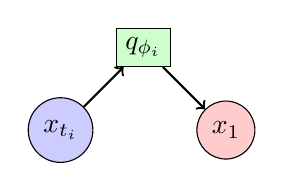
\begin{tikzpicture}[scale=0.7]
\node[draw, circle, fill=blue!20] (xti) at (0,0) {$x_{t_i}$};
\node[draw, circle, fill=red!20] (x1) at (3,0) {$x_1$};
\node[draw, rectangle, fill=green!20] (gen) at (1.5,1.5) {$q_{\phi_i}$};
\draw[->, thick] (xti) -- (gen);
\draw[->, thick] (gen) -- (x1);
\end{tikzpicture}
\end{center}
\end{column}
\end{columns}

\vspace{0.3cm}
\begin{alertblock}{Objective}
Optimize $\phi_i$ such that $q_{\phi_i}(x_1|x_{t_i}) = p(x_1|x_{t_i})$
\end{alertblock}

\begin{alertblock}{Why predict $x_1$?}
We only have access to real samples from $\pi_1$, not intermediate
states $p(x_t)$.
Thus, $p(x_1\mid x_{t_i})$ is the \textbf{only conditional distribution directly learnable}
from available data.
Once this conditional is learned, the true transition kernel
$p(x_{t_{i+1}}\mid x_{t_i})$
can be recovered by marginalizing over $x_1$ using the SB Gaussian bridge formula.
\end{alertblock}
\end{frame}

\section{Theorem 1: Optimization Objective}

\begin{frame}{Theorem 1: Constrained Optimization}
\begin{block}{Where does the loss come from?}
The objective in (9)--(10) is a discretized form of the SB variational principle:
\[
\min \; \mathbb{E}[\text{transport cost}] - \tau \cdot \text{entropy}.
\]
The energy term encourages $x_{t_i}$ and $x_1$ to align, while the entropy term ensures the stochasticity inherent in SB.
This mirrors entropy-regularized optimal transport.
\end{block}

\begin{theorem}[Core UNSB Theorem]
For any $t_i$, consider the following constrained optimization:
\begin{align}
\min_{\phi_i} \quad & \mathcal{L}_{\text{SB}}(\phi_i, t_i) := \mathbb{E}_{q_{\phi_i}(x_{t_i}, x_1)}[\|x_{t_i} - x_1\|^2] \notag \\
& \quad - 2\tau(1-t_i)\textcolor{blue}{H(q_{\phi_i}(x_{t_i}, x_1))} \tag{9} \\
\text{s.t.} \quad & \mathcal{L}_{\text{Adv}}(\phi_i, t_i) := D_{\text{KL}}(q_{\phi_i}(x_1) \| p(x_1)) = 0 \tag{10}
\end{align}
\end{theorem}

\begin{block}{Two Key Components}
\begin{enumerate}
    \item \textbf{SB Loss} $\mathcal{L}_{\text{SB}}$: Transport cost + entropy regularization
    \item \textbf{Adversarial Constraint} $\mathcal{L}_{\text{Adv}}$: Ensures marginal matching
\end{enumerate}
\end{block}
\end{frame}

\begin{frame}{Understanding the SB Loss}
\begin{equation}
\mathcal{L}_{\text{SB}}(\phi_i, t_i) = \underbrace{\mathbb{E}[\|x_{t_i} - x_1\|^2]}_{\text{Transport Cost}} - \underbrace{2\tau(1-t_i)H(q_{\phi_i}(x_{t_i}, x_1))}_{\text{Entropy Regularization}}
\end{equation}

\begin{columns}
\begin{column}{0.5\textwidth}
\textbf{Transport cost:}
\begin{itemize}
    \item Encourages $x_{t_i}$ close to $x_1$
    \item Minimizes expected squared distance
    \item Similar to Optimal Transport
\end{itemize}
\end{column}

\begin{column}{0.5\textwidth}
\textbf{Entropy regularization:}
\begin{itemize}
    \item \textcolor{blue}{$H(\cdot)$}: Joint entropy
    \item \textcolor{blue}{$\tau$}: Temperature parameter
    \item \textcolor{blue}{$(1-t_i)$}: Time weight
    \item Encourages \alert{diversity}
\end{itemize}
\end{column}
\end{columns}

\vspace{0.3cm}
\begin{alertblock}{Trade-off}
$\tau \uparrow$ $\Rightarrow$ More stochastic mapping \quad | \quad $\tau \downarrow$ $\Rightarrow$ More deterministic
\end{alertblock}

\pause
\vspace{0.3cm}
\textbf{Question:} What happens if we remove entropy regularization ($\tau = 0$)?
\end{frame}

\begin{frame}{Why Entropy Regularization?}
\begin{block}{Without Entropy ($\tau = 0$)}
\begin{equation}
\min \mathbb{E}[\|x_{t_i} - x_1\|^2] \quad \Rightarrow \quad \text{Deterministic Optimal Transport}
\end{equation}
Result: Each $x_0$ maps to a unique $x_1$ (mode collapse)
\end{block}

\pause
\begin{block}{With Entropy ($\tau > 0$)}
\begin{equation}
\min \mathbb{E}[\|x_{t_i} - x_1\|^2] - \tau H(q) \quad \Rightarrow \quad \text{Stochastic Bridge}
\end{equation}
Result: Each $x_0$ maps to a distribution $p(x_1|x_0)$
\end{block}

\pause
\vspace{0.3cm}
\textbf{Time-dependent weight:} $(1-t_i)$
\begin{itemize}
    \item \textbf{Early stage} ($t_i$ small): High entropy $\Rightarrow$ exploration
    \item \textbf{Late stage} ($t_i \rightarrow 1$): Low entropy $\Rightarrow$ convergence
\end{itemize}

\pause
\vspace{0.3cm}
\textbf{Analogy:} Similar to annealing - high temperature (early) for exploration, low temperature (late) for refinement
\end{frame}

\begin{frame}{Computing Entropy in High Dimensions}
\textbf{Problem:} For 256×256 images, direct entropy computation is intractable!

\pause
\begin{block}{Solution: Energy-Based Model Approximation}
Define energy network $E_\psi(x_{t_i}, x_1)$ such that:
\begin{equation}
q(x_{t_i}, x_1) = \frac{\exp(-E_\psi(x_{t_i}, x_1))}{Z_\psi}
\end{equation}

Then entropy can be approximated:
\begin{equation}
H(q) \approx \mathbb{E}_q[E_\psi(x_{t_i}, x_1)] + \log Z_\psi
\end{equation}
\end{block}

\pause
\textbf{Training strategy:}
\begin{itemize}
    \item \textcolor{blue}{Positive pairs}: $(x_{t_i}, x_1)$ from same trajectory $\rightarrow$ high energy
    \item \textcolor{red}{Negative pairs}: $(x_{t_i}, x_1')$ from different trajectories $\rightarrow$ low energy
    \item Use \texttt{logsumexp} for numerically stable $\log Z_\psi$ approximation
\end{itemize}

\pause
\vspace{0.3cm}
\textbf{Question:} How does this contrastive approach help estimate entropy?
\end{frame}

\begin{frame}{The Adversarial Constraint}
\begin{equation}
\mathcal{L}_{\text{Adv}}(\phi_i, t_i) := D_{\text{KL}}(q_{\phi_i}(x_1) \| p(x_1)) = 0
\end{equation}

\begin{block}{Meaning}
The marginal distribution $q_{\phi_i}(x_1)$ must match the true target distribution $p(x_1)$
\end{block}

\pause
\textbf{Why KL = 0 (exact matching)?}
\begin{itemize}
    \item Strong constraint: requires \alert{perfect distribution match}
    \item In practice: approximated via GAN training
    \item Theorem 1 proof requires exact marginal matching
\end{itemize}

\pause
\vspace{0.3cm}
\begin{columns}
\begin{column}{0.5\textwidth}
\textbf{Generator objective:}
\begin{itemize}
    \item Minimize $\mathcal{L}_{\text{SB}}$
    \item Fool discriminator
\end{itemize}
\end{column}

\begin{column}{0.5\textwidth}
\textbf{Discriminator objective:}
\begin{itemize}
    \item Distinguish $q_{\phi_i}(x_1)$ from $p(x_1)$
    \item Enforce marginal constraint
\end{itemize}
\end{column}
\end{columns}

\pause
\vspace{0.3cm}
\textbf{Question:} Can we relax this to $D_{\text{KL}} \approx 0$ in practice?
\end{frame}

\begin{frame}{Gaussian Transition Kernel}
\textbf{Key insight:} SB optimal process is closest to Brownian motion

Define transition distribution:
\begin{equation}
p(x_{t_{i+1}}|x_1, x_{t_i}) := \mathcal{N}\left(x_{t_{i+1}}\mid s_{i+1}x_1 + (1-s_{i+1})x_{t_i}, \textcolor{blue}{s_{i+1}(1-s_{i+1})\tau(1-t_i)}I\right)
\end{equation}
where $s_{i+1} := \frac{t_{i+1} - t_i}{1 - t_i}$

\pause
\begin{block}{Induced Conditional Distribution}
\begin{equation}
q_{\phi_i}(x_{t_{i+1}}|x_{t_i}) := \mathbb{E}_{q_{\phi_i}(x_1|x_{t_i})}[p(x_{t_{i+1}}|x_1, x_{t_i})]
\end{equation}
\end{block}

\pause
\textbf{Understanding the distribution:}
\begin{itemize}
    \item \textbf{Mean}: $s_{i+1}x_1 + (1-s_{i+1})x_{t_i}$ interpolates between current and endpoint
    \item \textbf{Variance}: $s_{i+1}(1-s_{i+1})\tau(1-t_i)$ varies with time
    \item This is discretization of Ornstein-Uhlenbeck process
\end{itemize}

\pause
\begin{block}{Interpretation of the Gaussian bridge}
The mean
\[
s_{i+1}x_1 + (1-s_{i+1})x_{t_i}
\]
describes a \textbf{linear interpolation} between current and final state.

The variance
\[
s_{i+1}(1-s_{i+1})\tau(1-t_i)
\]
expresses the \textbf{uncertainty of a Brownian bridge}, which must vanish at $t=1$ and be largest in the middle.

Thus equation (11) is exactly the conditional law of a Brownian bridge conditioned on $x_{t_i}$ and $x_1$.
\end{block}

\pause
\vspace{0.3cm}
\textbf{Question:} Why take expectation over $x_1$ instead of using a fixed endpoint?

\pause
\begin{alertblock}{Why average over $x_1$?}
The bridge dynamics from $t_i$ to $t_{i+1}$ depend on the unknown future endpoint.
In SB theory the correct transition is obtained by marginalizing the bridge kernel:
\[
p(x_{t_{i+1}}\mid x_{t_i})
 = \mathbb{E}_{p(x_1\mid x_{t_i})}[p(x_{t_{i+1}}\mid x_{t_i},x_1)].
\]
Thus UNSB follows the \textbf{exact} SB decomposition.
\end{alertblock}
\end{frame}

\begin{frame}{Theorem 1 Conclusion}
\begin{theorem}[Continued]
If $\phi_i$ solves the optimization problem (Eq. 9-10), then:
\begin{equation}
\boxed{
\begin{aligned}
q_{\phi_i}(x_1|x_{t_i}) &= p(x_1|x_{t_i}) \\
q_{\phi_i}(x_{t_{i+1}}|x_{t_i}) &= p(x_{t_{i+1}}|x_{t_i}) \\
q_{\phi_i}(x_{t_{i+1}}) &= p(x_{t_{i+1}})
\end{aligned}
}
\end{equation}
\end{theorem}

\pause
\begin{alertblock}{Power of the Theorem}
\begin{enumerate}
    \item Learned generator $q_{\phi_i}$ exactly recovers true SB posterior $p(x_1|x_{t_i})$
    \item Induced next-step distribution $q_{\phi_i}(x_{t_{i+1}}|x_{t_i})$ is also correct
    \item Marginal distribution $q_{\phi_i}(x_{t_{i+1}})$ matches true distribution
\end{enumerate}
\end{alertblock}

\pause
\vspace{0.2cm}
\textcolor{blue}{\textbf{Recursive application}}: With $p(x_{t_{i+1}})$, we can learn $p(x_{t_{i+2}}|x_{t_{i+1}})$, and so on!

\pause
\vspace{0.3cm}
\textbf{Key insight:} Learn endpoint prediction $\Rightarrow$ automatically get entire Markov chain

\pause
\begin{block}{Meaning of the theorem}
If the endpoint predictor $q_{\phi_i}(x_1\mid x_{t_i})$ is learned perfectly,
then the entire Markov chain of the SB is recovered automatically:
\begin{itemize}
    \item the true posterior $p(x_1\mid x_{t_i})$,
    \item the true transition kernel $p(x_{t_{i+1}}\mid x_{t_i})$,
    \item and the true marginal $p(x_{t_{i+1}})$.
\end{itemize}
This shows that \textbf{learning only endpoint predictions is sufficient} to reconstruct the whole stochastic process.
\end{block}
\end{frame}

\section{Generation–Training Dual-Stage Mechanism}

\begin{frame}{Why Two Stages? A Structural View}
UNSB separates the learning dynamics into a \textbf{generation stage} and a \textbf{training stage}.
Although the Markov chain $p(x_{t_{j+1}}|x_{t_j})$ can be simulated once the conditional generator
$q_{\phi_i}(x_1|x_{t_j})$ is available, this does \emph{not} imply that training is unnecessary after generation.
Instead, the two stages serve fundamentally different purposes.

\begin{itemize}
    \item \textbf{Generation Stage:}
    Simulates the forward SB trajectory using the current generator.
    No gradients are allowed to flow through the chain (``stop–gradient''),
    ensuring unbiased intermediate samples.

    \item \textbf{Training Stage:}
    Uses the generated samples to compute the OT+entropy objective and the adversarial constraint.
    Updates the generator to better approximate $p(x_1|x_{t_i})$.
\end{itemize}

Critically, the Markov chain generated so far is \emph{not} correct SB dynamics; it reflects the
current generator, not the optimal one. Training must refine $q_{\phi_i}$ iteratively.
\end{frame}

\begin{frame}{Generation vs. Training: Side-by-Side Comparison}
\begin{table}
\small
\begin{tabular}{p{3cm}p{5cm}p{5cm}}
\toprule
\textbf{Aspect} & \textbf{Generation Stage} & \textbf{Training Stage} \\
\midrule
\textbf{Purpose} &
Sample intermediate states &
Optimize generator parameters \\
\midrule
\textbf{Gradient} &
Stop-gradient (detached) &
Full backpropagation \\
\midrule
\textbf{Input} &
$x_0 \sim \pi_0$, current $q_{\phi}$ &
Generated $(x_{t_i}, x_1)$ pairs \\
\midrule
\textbf{Output} &
Trajectory $\{x_{t_j}\}_{j=0}^{i}$ &
Updated $\phi_i$ \\
\midrule
\textbf{Computational role} &
Forward simulation (inference-like) &
Loss computation + optimization \\
\midrule
\textbf{Frequency} &
Every minibatch &
Every minibatch \\
\bottomrule
\end{tabular}
\end{table}

\pause
\vspace{0.3cm}
\textbf{Key insight:} Generation is \alert{not inference}—it's a mechanism to create training data for local conditionals.
\end{frame}

\begin{frame}{The Role of the Generation Stage}
\begin{block}{Purpose}
Generate unbiased intermediate states $\{x_{t_j}\}_{j=0}^{i}$ required to evaluate
the objective for time step $t_i$.
\end{block}

Given $x_0 \sim \pi_0$, UNSB performs:
\begin{equation}
x_{t_{j+1}}
\sim q_{\phi}(x_{t_{j+1}}|x_{t_j})
= \mathbb{E}_{q_{\phi}(x_1|x_{t_j})}
\left[
p(x_{t_{j+1}}|x_1, x_{t_j})
\right],
\end{equation}
where the Gaussian kernel $p(\cdot|\cdot)$ corresponds to the local OU transition.

\textbf{Key constraints:}
\begin{itemize}
    \item No gradient flows through sampling.
    \item Generated $x_{t_j}$ represents the \emph{current} approximation of SB marginals.
    \item These samples enable the conditional loss and KL constraint at time $t_i$.
\end{itemize}

The generation stage is therefore a \textbf{rollout} of the current model, not the final system.
\end{frame}

\begin{frame}{Why Stop-Gradient is Essential}
\begin{alertblock}{Mathematical necessity of detachment}
If we allow gradients to flow through the entire chain $x_0 \rightarrow x_{t_1} \rightarrow \cdots \rightarrow x_{t_i}$,
we face two critical problems:
\end{alertblock}

\pause
\textbf{Problem 1: Computational explosion}
\begin{itemize}
    \item Memory cost grows linearly with $i$ (number of time steps traversed)
    \item Gradient computation requires storing all intermediate activations
    \item For $i=4$ and image size $256\times256$, memory $\sim 4\times$ batch size
\end{itemize}

\pause
\textbf{Problem 2: Biased gradient estimates}
\begin{itemize}
    \item The chain $\{x_{t_j}\}$ is a \textbf{stochastic rollout}
    \item Backprop through stochastic sampling introduces high variance
    \item The gradient w.r.t. $\phi_i$ should reflect $p(x_1|x_{t_i})$, not the entire path distribution
\end{itemize}

\pause
\begin{block}{Solution: Stop-gradient}
Treat $x_{t_j}$ ($j < i$) as \textbf{fixed samples} from $q_{\phi}(x_{t_j})$,
allowing unbiased estimation of $\mathcal{L}_{SB}(\phi_i, t_i)$.
\end{block}
\end{frame}

\begin{frame}{The Role of the Training Stage}
\textbf{Generation alone cannot improve the model.}
It merely simulates what the current $q_{\phi_i}$ produces.
To improve $q_{\phi_i}$, the UNSB framework must evaluate two core terms:

\begin{itemize}
    \item \textbf{OT + entropy loss} (Eq. 9)
    \item \textbf{Marginal-matching adversarial constraint} (Eq. 10)
\end{itemize}

During the training stage, we compute:
\begin{equation}
\mathcal{L}_{SB}(\phi_i,t_i) =
\mathbb{E}_{q_{\phi_i}(x_{t_i},x_1)}
\left[\|x_{t_i}-x_1\|^2\right]
- 2\tau(1-t_i)H(q_{\phi_i}),
\end{equation}
and enforce:
\begin{equation}
D_{KL}\left(q_{\phi_i}(x_1)\,\|\,p(x_1)\right)=0.
\end{equation}

Only the training stage updates the generator, gradually making the Markov chain closer to the
true SB dynamics.
\end{frame}

\begin{frame}{Figure 3 Visualization: Dual-Stage Mechanism}
\begin{center}
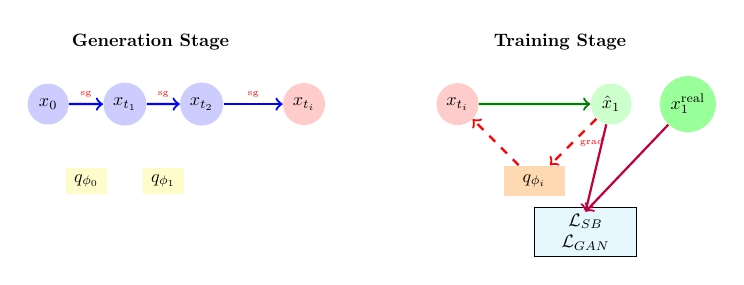
\begin{tikzpicture}[scale=0.65, transform shape]
% Generation Stage (Left)
\node[anchor=north] at (-4,4) {\textbf{Generation Stage}};
\node[circle, fill=blue!20, minimum size=0.8cm] (x0) at (-6,2.5) {$x_0$};
\node[circle, fill=blue!20, minimum size=0.8cm] (xt1) at (-4.5,2.5) {$x_{t_1}$};
\node[circle, fill=blue!20, minimum size=0.8cm] (xt2) at (-3,2.5) {$x_{t_2}$};
\node[circle, fill=red!20, minimum size=0.8cm] (xti) at (-1,2.5) {$x_{t_i}$};

% Generators for generation
\node[rectangle, fill=yellow!20, minimum width=0.8cm, minimum height=0.5cm] (g0) at (-5.25,1) {$q_{\phi_0}$};
\node[rectangle, fill=yellow!20, minimum width=0.8cm, minimum height=0.5cm] (g1) at (-3.75,1) {$q_{\phi_1}$};

% Arrows with sg labels
\draw[->, thick, blue] (x0) -- (xt1) node[midway, above, red, font=\tiny] {sg};
\draw[->, thick, blue] (xt1) -- (xt2) node[midway, above, red, font=\tiny] {sg};
\draw[->, thick, blue] (xt2) -- (xti) node[midway, above, red, font=\tiny] {sg};

% Training Stage (Right)
\node[anchor=north] at (4,4) {\textbf{Training Stage}};
\node[circle, fill=red!20, minimum size=0.8cm] (xti2) at (2,2.5) {$x_{t_i}$};
\node[circle, fill=green!20, minimum size=0.8cm] (x1) at (5,2.5) {$\hat{x}_1$};
\node[rectangle, fill=orange!30, minimum width=1.2cm, minimum height=0.6cm] (gi) at (3.5,1) {$q_{\phi_i}$};

% Real sample
\node[circle, fill=green!40, minimum size=0.8cm] (x1real) at (6.5,2.5) {$x_1^{\text{real}}$};

% Arrows with gradient
\draw[->, thick, green!50!black] (xti2) -- (x1);
\draw[->, thick, red, dashed] (x1) -- (gi) node[midway, right, font=\tiny] {grad};
\draw[->, thick, red, dashed] (gi) -- (xti2);

% Loss computation
\node[rectangle, draw, fill=cyan!10, minimum width=2cm, minimum height=0.8cm, align=center] at (4.5,0) {$\mathcal{L}_{SB}$\\$\mathcal{L}_{GAN}$};

% Discriminator
\draw[->, thick, purple] (x1) -- (4.5,0.4);
\draw[->, thick, purple] (x1real) -- (4.5,0.4);
\end{tikzpicture}
\end{center}

\textbf{Left (Generation):} Forward rollout with stop-gradient (sg) at each step.

\textbf{Right (Training):} Backpropagation only through $q_{\phi_i}$, using generated $x_{t_i}$ and real $x_1^{\text{real}}$.
\end{frame}

\begin{frame}{Data Flow vs. Gradient Flow}
\begin{center}
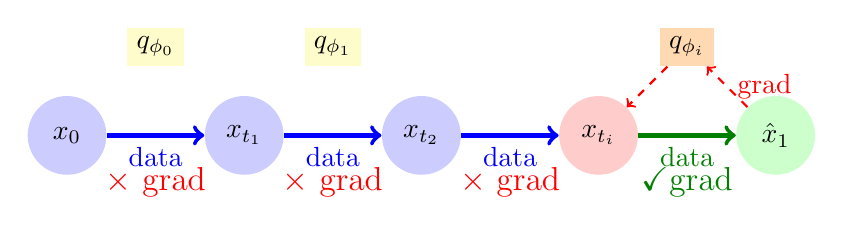
\begin{tikzpicture}[scale=0.75]
% Nodes
\node[circle, fill=blue!20, minimum size=1cm] (x0) at (0,0) {$x_0$};
\node[circle, fill=blue!20, minimum size=1cm] (xt1) at (3,0) {$x_{t_1}$};
\node[circle, fill=blue!20, minimum size=1cm] (xt2) at (6,0) {$x_{t_2}$};
\node[circle, fill=red!20, minimum size=1cm] (xti) at (9,0) {$x_{t_i}$};
\node[circle, fill=green!20, minimum size=1cm] (x1) at (12,0) {$\hat{x}_1$};

% Generators
\node[rectangle, fill=yellow!20] (g0) at (1.5,1.5) {$q_{\phi_0}$};
\node[rectangle, fill=yellow!20] (g1) at (4.5,1.5) {$q_{\phi_1}$};
\node[rectangle, fill=orange!30] (gi) at (10.5,1.5) {$q_{\phi_i}$};

% Data flow (solid arrows)
\draw[->, ultra thick, blue] (x0) -- (xt1) node[midway, below] {data};
\draw[->, ultra thick, blue] (xt1) -- (xt2) node[midway, below] {data};
\draw[->, ultra thick, blue] (xt2) -- (xti) node[midway, below] {data};
\draw[->, ultra thick, green!50!black] (xti) -- (x1) node[midway, below] {data};

% Gradient flow (dashed arrows, only for training stage)
\draw[->, thick, red, dashed] (x1) -- (gi) node[midway, right] {grad};
\draw[->, thick, red, dashed] (gi) -- (xti);

% Stop-gradient markers
\node[red] at (1.5,-0.8) {\large $\times$ grad};
\node[red] at (4.5,-0.8) {\large $\times$ grad};
\node[red] at (7.5,-0.8) {\large $\times$ grad};
\node[green!50!black] at (10.5,-0.8) {\large \checkmark grad};
\end{tikzpicture}
\end{center}

\textbf{Interpretation:}
\begin{itemize}
    \item \textcolor{blue}{Solid blue arrows}: Data flows forward through entire chain
    \item \textcolor{red}{Dashed red arrows}: Gradients only backprop through $q_{\phi_i}$
    \item \textcolor{red}{$\times$ markers}: Stop-gradient operations
    \item \textcolor{green!50!black}{\checkmark marker}: Gradient allowed
\end{itemize}
\end{frame}

\begin{frame}{Why Generation Cannot Replace Training}
A common misunderstanding is believing that if $x_{t_{j+1}}$ can be generated, training is redundant.
However:

\begin{alertblock}{Generation produces samples; training adjusts the model.}
\end{alertblock}

\begin{itemize}
    \item Generated states depend on the \emph{current} $q_{\phi_i}$, not the optimal one.
    \item Without training, the process collapses to trivial deterministic mappings.
    \item Entropy term cannot be computed without joint samples from the generator.
    \item The adversarial marginal constraint requires discriminator feedback.
\end{itemize}

\textbf{Therefore, generation ≠ learning.}
Training uses generated states to refine $q_{\phi_i}$ so that the next generation stage is more accurate.
\end{frame}

\begin{frame}{The Bootstrap Loop: How Quality Improves}
\begin{center}
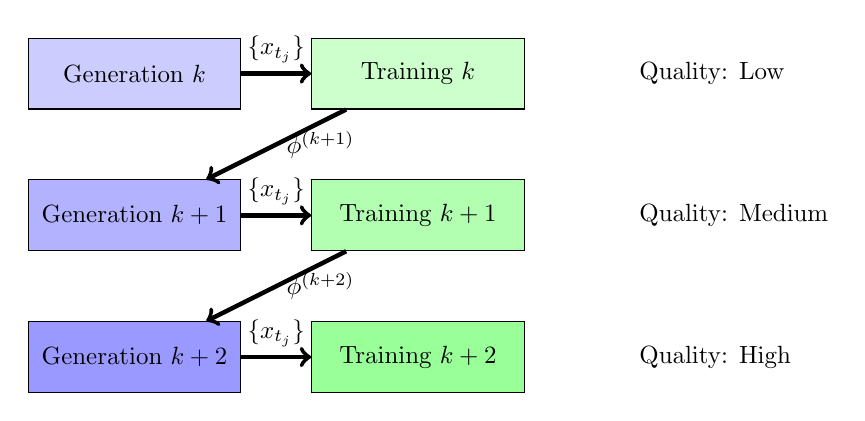
\begin{tikzpicture}[scale=0.9, transform shape]
% Iteration 1
\node[draw, rectangle, fill=blue!20, minimum width=3cm, minimum height=1cm] (gen1) at (0,3) {Generation $k$};
\node[draw, rectangle, fill=green!20, minimum width=3cm, minimum height=1cm] (train1) at (4,3) {Training $k$};

% Iteration 2
\node[draw, rectangle, fill=blue!30, minimum width=3cm, minimum height=1cm] (gen2) at (0,1) {Generation $k+1$};
\node[draw, rectangle, fill=green!30, minimum width=3cm, minimum height=1cm] (train2) at (4,1) {Training $k+1$};

% Iteration 3
\node[draw, rectangle, fill=blue!40, minimum width=3cm, minimum height=1cm] (gen3) at (0,-1) {Generation $k+2$};
\node[draw, rectangle, fill=green!40, minimum width=3cm, minimum height=1cm] (train3) at (4,-1) {Training $k+2$};

% Arrows
\draw[->, ultra thick] (gen1) -- (train1) node[midway, above] {$\{x_{t_j}\}$};
\draw[->, ultra thick] (train1) -- (gen2) node[midway, right] {$\phi^{(k+1)}$};
\draw[->, ultra thick] (gen2) -- (train2) node[midway, above] {$\{x_{t_j}\}$};
\draw[->, ultra thick] (train2) -- (gen3) node[midway, right] {$\phi^{(k+2)}$};
\draw[->, ultra thick] (gen3) -- (train3) node[midway, above] {$\{x_{t_j}\}$};

% Quality indicators
\node[right] at (7,3) {Quality: Low};
\node[right] at (7,1) {Quality: Medium};
\node[right] at (7,-1) {Quality: High};
\end{tikzpicture}
\end{center}

\pause
\textbf{Convergence property:}
\begin{itemize}
    \item As $k \rightarrow \infty$, $q_{\phi_i}^{(k)}(x_1|x_{t_i}) \rightarrow p(x_1|x_{t_i})$
    \item Generated samples $\{x_{t_j}\}^{(k)}$ approach true SB marginals $p(x_{t_j})$
    \item This bootstrapping is provably stable under Theorem 1's conditions
\end{itemize}
\end{frame}

\begin{frame}{Why Don't Diffusion Models Need This Dual-Stage Mechanism?}
\textbf{Question:} Diffusion models also have forward and reverse processes. Why don't they use UNSB's dual-stage approach?

\pause
\begin{columns}
\begin{column}{0.5\textwidth}
\textbf{Diffusion Models:}
\begin{itemize}
    \item \textcolor{blue}{Forward process is fixed} (Gaussian noise)
    \item No need to generate training data
    \item Learn only reverse process $p_\theta(x_{t-1}|x_t)$
    \item Directly train on $x_t = \sqrt{\bar{\alpha}_t}x_0 + \sqrt{1-\bar{\alpha}_t}\epsilon$
\end{itemize}
\end{column}

\begin{column}{0.5\textwidth}
\textbf{UNSB:}
\begin{itemize}
    \item \textcolor{red}{Forward process is learned}
    \item Must generate $x_{t_i}$ from $\pi_0$
    \item Learn conditionals $q(x_1|x_{t_i})$
    \item Cannot directly sample $x_{t_i}$ without simulation
\end{itemize}
\end{column}
\end{columns}

\pause
\vspace{0.3cm}
\begin{alertblock}{Key difference}
UNSB learns a \textbf{bidirectional bridge} between arbitrary $\pi_0$ and $\pi_1$,
requiring generation to produce intermediate samples.
Diffusion models learn a \textbf{unidirectional denoising} process with a fixed forward path.
\end{alertblock}
\end{frame}

\begin{frame}{Why Must Training Be Performed at Every Time Step?}
UNSB optimizes local conditionals:
\begin{equation}
p(x_1|x_{t_i}) \qquad \forall i = 0,1,\dots,N-1.
\end{equation}

This requires:
\begin{itemize}
    \item Intermediate samples at exactly time $t_i$.
    \item A fresh forward rollout for every minibatch.
    \item Computing entropy over $(x_{t_i},x_1)$ pairs.
    \item Comparing the predicted marginal $q_{\phi_i}(x_1)$ with $\pi_1$ using GAN loss.
\end{itemize}

If training is skipped at some time index:
\begin{itemize}
    \item The local conditional fails to converge.
    \item The induced Markov chain deviates from the true SB dynamics.
    \item Errors accumulate and destroy the bridge structure.
\end{itemize}

This mirrors classical SB: local consistency ensures global correctness.
\end{frame}

\begin{frame}{Detailed Algorithm: Dual-Stage in Practice}
\begin{algorithm}[H]
\small
\caption{UNSB Dual-Stage Training (Single Iteration)}
\begin{algorithmic}[1]
\STATE Sample $x_0 \sim \pi_0$, $x_1^{\text{real}} \sim \pi_1$
\STATE Randomly select time index $t_i \in \{t_0, t_1, \ldots, t_{N-1}\}$
\STATE
\STATE \textcolor{blue}{// === Generation Stage (Stop-Gradient) ===}
\STATE $x_{t_0} \leftarrow x_0$
\FOR{$j = 0$ to $i-1$}
    \STATE $\hat{x}_1^{(j)} \leftarrow q_{\phi_j}(x_1|x_{t_j})$ with noise $z \sim \mathcal{N}(0,I)$
    \STATE $x_{t_{j+1}} \leftarrow s_{j+1}\hat{x}_1^{(j)} + (1-s_{j+1})x_{t_j} + \sqrt{s_{j+1}(1-s_{j+1})\tau(1-t_j)}\epsilon$
    \STATE $x_{t_{j+1}} \leftarrow \text{detach}(x_{t_{j+1}})$ \textcolor{red}{// Stop gradient!}
\ENDFOR
\STATE
\STATE \textcolor{blue}{// === Training Stage (Full Gradient) ===}
\STATE $\hat{x}_1^{(i)} \leftarrow q_{\phi_i}(x_1|x_{t_i})$ with noise $z \sim \mathcal{N}(0,I)$
\STATE Compute $\mathcal{L}_{SB} = \|x_{t_i} - \hat{x}_1^{(i)}\|^2 - 2\tau(1-t_i)H(x_{t_i}, \hat{x}_1^{(i)})$
\STATE Compute $\mathcal{L}_{GAN}$ using discriminator $D(\hat{x}_1^{(i)})$ vs. $D(x_1^{\text{real}})$
\STATE Update $\phi_i$ via $\nabla_{\phi_i}(\lambda_{SB}\mathcal{L}_{SB} + \lambda_{GAN}\mathcal{L}_{GAN})$
\end{algorithmic}
\end{algorithm}
\end{frame}

\begin{frame}{Theoretical Guarantee: Why This Mechanism Works}
\begin{theorem}[Convergence of Dual-Stage Training]
Under the following conditions:
\begin{enumerate}
    \item Generators $q_{\phi_i}$ have sufficient capacity
    \item Adversarial constraint is satisfied: $D_{KL}(q_{\phi_i}(x_1) \| p(x_1)) = 0$
    \item Stop-gradient prevents bias accumulation
\end{enumerate}
The dual-stage mechanism converges to the true SB solution:
\begin{equation}
\lim_{k\rightarrow\infty} q_{\phi_i}^{(k)}(x_1|x_{t_i}) = p^*(x_1|x_{t_i}),
\end{equation}
where $p^*$ is the optimal Schrödinger Bridge.
\end{theorem}

\pause
\vspace{0.3cm}
\textbf{Proof sketch:}
\begin{itemize}
    \item Each time step $t_i$ optimizes a local SB subproblem
    \item Markov property ensures global consistency from local optimality
    \item Iterative refinement follows a contraction mapping (similar to Sinkhorn)
\end{itemize}
\end{frame}

\begin{frame}{Common Misconceptions About the Dual-Stage Mechanism}
\begin{enumerate}
    \item \textbf{Misconception:} ``Generation stage is just inference.''
    \begin{itemize}
        \item \textcolor{red}{Wrong:} Inference produces final $x_1$ from $x_0$
        \item \textcolor{green!50!black}{Correct:} Generation produces intermediate $x_{t_i}$ for training
    \end{itemize}

    \pause
    \item \textbf{Misconception:} ``We can train once and generate forever.''
    \begin{itemize}
        \item \textcolor{red}{Wrong:} Generator is learned, not given
        \item \textcolor{green!50!black}{Correct:} Training iteratively improves generation quality
    \end{itemize}

    \pause
    \item \textbf{Misconception:} ``Stop-gradient is for memory efficiency only.''
    \begin{itemize}
        \item \textcolor{red}{Wrong:} It's also theoretically necessary
        \item \textcolor{green!50!black}{Correct:} Prevents biased gradient estimates and ensures correct SB learning
    \end{itemize}

    \pause
    \item \textbf{Misconception:} ``This is the same as GAN training.''
    \begin{itemize}
        \item \textcolor{red}{Wrong:} GANs don't have time-indexed conditionals
        \item \textcolor{green!50!black}{Correct:} UNSB learns a sequence of time-dependent generators $\{q_{\phi_i}\}$
    \end{itemize}
\end{enumerate}
\end{frame}

\begin{frame}{Computational Cost Analysis}
\textbf{Per-iteration complexity:}

\begin{table}
\small
\begin{tabular}{lcc}
\toprule
\textbf{Operation} & \textbf{Time Complexity} & \textbf{Memory} \\
\midrule
Generation stage & $O(i \cdot C_{forward})$ & $O(1)$ (detached) \\
Training stage & $O(C_{forward} + C_{backward})$ & $O(B \cdot d)$ \\
Discriminator & $O(C_D)$ & $O(B \cdot d_D)$ \\
Energy network & $O(C_E)$ & $O(B \cdot d_E)$ \\
\midrule
\textbf{Total} & $O(i \cdot C_{forward} + C_{backward})$ & $O(B \cdot d)$ \\
\bottomrule
\end{tabular}
\end{table}

where:
\begin{itemize}
    \item $i$: Number of time steps to reach $t_i$ (typically $\leq 5$)
    \item $C_{forward}$: Cost of one generator forward pass
    \item $C_{backward}$: Cost of backpropagation
    \item $B$: Batch size, $d$: Data dimension
\end{itemize}

\pause
\vspace{0.3cm}
\textbf{Key observation:} Stop-gradient keeps memory $O(B \cdot d)$ instead of $O(i \cdot B \cdot d)$
\end{frame}

\begin{frame}{Summary of the Dual-Stage Mechanism}
\textbf{Generation stage:}
\begin{itemize}
    \item Produces unbiased intermediate $x_{t_j}$.
    \item Strictly stop-gradient.
    \item Models the current bridge approximation.
\end{itemize}

\textbf{Training stage:}
\begin{itemize}
    \item Computes OT+entropy loss.
    \item Enforces adversarial marginal matching.
    \item Updates the generator.
\end{itemize}

\begin{alertblock}{Together they form a bootstrapping loop:}
Generation provides samples → training improves the model →
better model produces better samples → repeat.
\end{alertblock}

This mechanism is essential because SB is a \textbf{global optimal transport problem}
solved through \textbf{local conditional learning}.
\end{frame}

\begin{frame}{Final Summary: Why Both Stages are Necessary}
\begin{block}{Why both stages are necessary}
\begin{enumerate}
    \item \textbf{Generation:} Creates intermediate samples $x_{t_i}$ that cannot be directly sampled from $\pi_0$ or $\pi_1$
    \item \textbf{Training:} Optimizes local conditionals $q_{\phi_i}(x_1|x_{t_i})$ using these samples
    \item \textbf{Iteration:} Bootstraps from poor initial approximation to correct SB dynamics
\end{enumerate}
\end{block}

\pause
\begin{alertblock}{Design principles}
\begin{itemize}
    \item Stop-gradient: Ensures unbiased gradients and computational feasibility
    \item Local learning: Each $\phi_i$ optimized independently, but globally consistent via Markov property
    \item Adversarial constraint: Ensures marginal matching without paired data
\end{itemize}
\end{alertblock}

\pause
\vspace{0.3cm}
\textbf{This mechanism distinguishes UNSB from:}
\begin{itemize}
    \item Diffusion models (fixed forward process)
    \item GANs (no time decomposition)
    \item OT methods (deterministic, requires Sinkhorn)
\end{itemize}
\end{frame}

\section{Algorithm and Implementation}

\begin{frame}{Training Algorithm Overview}
\begin{algorithm}[H]
\small
\caption{UNSB Training}
\begin{algorithmic}[1]
\FOR{each training iteration}
    \STATE Sample $x_0 \sim \pi_0$ (source), $x_1 \sim \pi_1$ (target)
    \STATE Randomly select time step $t \in \{0, 1, \ldots, T-1\}$
    \STATE \textcolor{blue}{// Forward simulation (with gradient detachment)}
    \FOR{$i = 0$ to $t$}
        \STATE $X_{t_i} \leftarrow$ OU process update (detach)
        \STATE $\hat{X}_{t_i} \leftarrow G(X_{t_i}, t_i, z)$ (detach)
    \ENDFOR
    \STATE \textcolor{blue}{// Update discriminator}
    \STATE $\mathcal{L}_D \leftarrow$ LSGAN loss
    \STATE Update discriminator parameters
    \STATE \textcolor{blue}{// Update energy network}
    \STATE $\mathcal{L}_E \leftarrow$ Contrastive energy loss
    \STATE Update energy network parameters
    \STATE \textcolor{blue}{// Update generator}
    \STATE $\mathcal{L}_G \leftarrow \lambda_{\text{GAN}}\mathcal{L}_{\text{GAN}} + \lambda_{\text{SB}}\mathcal{L}_{\text{SB}} + \lambda_{\text{NCE}}\mathcal{L}_{\text{NCE}}$
    \STATE Update generator parameters
\ENDFOR
\end{algorithmic}
\end{algorithm}

\begin{block}{Why detach the forward simulation?}
The forward OU updates serve as \textbf{sampling of intermediate states},
not as trainable modules.
Detaching prevents gradients from flowing backward through the simulated
stochastic process, stabilizing training and reducing memory cost.
\end{block}
\end{frame}

\begin{frame}{Time Scheduling Strategy}
\textbf{Non-uniform time grid:}
\begin{equation}
\text{increments} = \left[0, 1, \frac{1}{2}, \frac{1}{3}, \ldots, \frac{1}{T-1}\right]
\end{equation}
Cumulative sum and normalize: emphasizes later time steps

\begin{center}
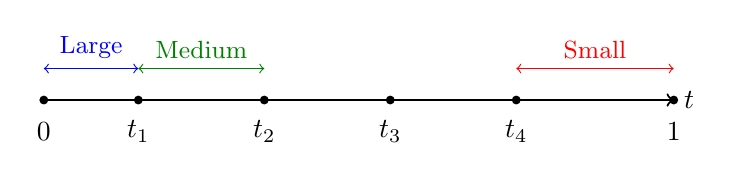
\begin{tikzpicture}[scale=0.8]
\draw[->, thick] (0,0) -- (10,0) node[right] {$t$};
\foreach \x in {0, 1.5, 3.5, 5.5, 7.5, 10}
    \fill (\x,0) circle (2pt);
\node at (0,-0.5) {$0$};
\node at (1.5,-0.5) {$t_1$};
\node at (3.5,-0.5) {$t_2$};
\node at (5.5,-0.5) {$t_3$};
\node at (7.5,-0.5) {$t_4$};
\node at (10,-0.5) {$1$};
\draw[<->, blue] (0,0.5) -- (1.5,0.5) node[midway, above] {\small Large};
\draw[<->, green!50!black] (1.5,0.5) -- (3.5,0.5) node[midway, above] {\small Medium};
\draw[<->, red] (7.5,0.5) -- (10,0.5) node[midway, above] {\small Small};
\end{tikzpicture}
\end{center}

\pause
\textbf{Rationale:}
\begin{itemize}
    \item \textbf{Early stage}: Large steps for rapid approach to target distribution
    \item \textbf{Late stage}: Small steps for fine-grained refinement
    \item Matches OU process characteristics
    \item Synergizes with time-decaying entropy weight $(1-t_i)$
\end{itemize}

\pause
\begin{block}{Harmonic schedule intuition}
Large steps at early times rapidly move samples
toward the target distribution.
Smaller steps near $t=1$ match the vanishing variance of the bridge
and allow fine refinement.
The schedule approximates the continuous-time SB in a few discrete steps.
\end{block}

\pause
\vspace{0.3cm}
\textbf{Question:} Why not use uniform spacing $t_i = i/T$?
\end{frame}

\begin{frame}{UNSB vs. Diffusion Models}
\begin{block}{Conceptual difference}
Diffusion models learn a reverse SDE by progressively denoising.
UNSB learns a small set of \textbf{direct stochastic transport maps}
and relies on SB theory rather than noise annealing.
\end{block}

\begin{columns}
\begin{column}{0.5\textwidth}
\textbf{Diffusion Models:}
\begin{itemize}
    \item Fixed forward process (noise)
    \item Learn reverse denoising
    \item Requires many time steps (1000+)
    \item Slow training and inference
    \item Usually need paired data
\end{itemize}
\end{column}

\begin{column}{0.5\textwidth}
\textbf{UNSB:}
\begin{itemize}
    \item Learned forward process
    \item Directly predict target $x_1$
    \item Few time steps (5)
    \item Fast training and inference
    \item \textcolor{blue}{No paired data}
\end{itemize}
\end{column}
\end{columns}

\pause
\vspace{0.3cm}
\textbf{Key differences:}
\begin{itemize}
    \item UNSB is \alert{bidirectional} (learns bridge $\pi_0 \rightarrow \pi_1$)
    \item Diffusion is unidirectional (noise $\rightarrow$ data)
    \item UNSB has theoretical optimality guarantees (Schrödinger Bridge)
\end{itemize}

\pause
\vspace{0.3cm}
\textbf{Question:} What enables UNSB to use so few time steps compared to diffusion?
\end{frame}

\begin{frame}{UNSB vs. CycleGAN}
\begin{columns}
\begin{column}{0.5\textwidth}
\textbf{CycleGAN:}
\begin{itemize}
    \item Cycle consistency: $F(G(x)) \approx x$
    \item \textcolor{red}{Assumption}: Mapping invertible
    \item Deterministic mapping
    \item May produce artifacts
    \item No theoretical optimality
\end{itemize}
\end{column}

\begin{column}{0.5\textwidth}
\textbf{UNSB:}
\begin{itemize}
    \item SB optimality
    \item \textcolor{blue}{No invertibility required}
    \item Stochastic mapping (more realistic)
    \item Smoother transitions
    \item Theoretical guarantees
\end{itemize}
\end{column}
\end{columns}

\pause
\vspace{0.3cm}
\textbf{Experimental comparison (MRI):}
\begin{itemize}
    \item UNSB SSIM: 0.82 vs CycleGAN: 0.78
    \item UNSB preserves more anatomical details
    \item UNSB generates more natural textures
\end{itemize}

\pause
\vspace{0.3cm}
\textbf{Question:} When would cycle consistency assumption be violated in practice?
\end{frame}

\section{Limited Paired Data: Hybrid Training}

\begin{frame}{When Limited Paired Data is Available}
\textbf{Scenario:} Most data is unpaired, but small amount of paired data exists

\pause
\begin{block}{Scheme A: SB GT Transport}
Add ground truth guidance within SB framework:
\begin{equation}
\mathcal{L}_{\text{SB}} \rightarrow \mathcal{L}_{\text{SB}} + \tau\|\hat{X}_t - X_{\text{GT}}\|^2
\end{equation}
\end{block}

\pause
\textbf{Key advantages:}
\begin{itemize}
    \item Maintains SB mathematical structure
    \item Coefficient $\tau$ consistent with entropy regularization
    \item GT guidance naturally integrated as additional transport cost
    \item Doesn't break theoretical guarantees
\end{itemize}

\pause
\begin{block}{Why GT term integrates cleanly}
The added term
\[
\tau\|\hat{X}_t - X_{\text{GT}}\|^2
\]
is another transport cost in the SB objective.
It does not break the stochastic nature or theoretical structure of the SB.
This is why paired data can be incorporated consistently.
\end{block}

\pause
\vspace{0.3cm}
\textbf{Two-stage training strategy:}
\begin{enumerate}
    \item \textbf{Stage 1 (Unpaired):} Learn from abundant unpaired data
    \begin{equation}
    \min \mathcal{L}_{\text{SB}} + \lambda_{\text{GAN}}\mathcal{L}_{\text{GAN}} + \lambda_{\text{NCE}}\mathcal{L}_{\text{NCE}}
    \end{equation}
    \item \textbf{Stage 2 (Paired fine-tuning):} Refine with limited paired data
    \begin{equation}
    \min \mathcal{L}_{\text{SB}} + \tau\|\hat{X}_t - X_{\text{GT}}\|^2 + \lambda_{\text{GAN}}\mathcal{L}_{\text{GAN}}
    \end{equation}
\end{enumerate}
\end{frame}

\begin{frame}{Unpaired + Paired Two-Stage Training}
\begin{center}
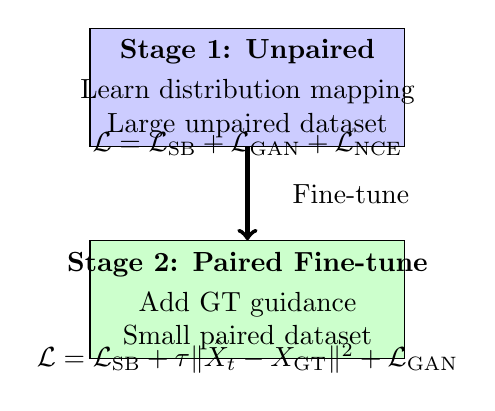
\begin{tikzpicture}[scale=0.9]
% Stage 1
\node[draw, rectangle, fill=blue!20, minimum width=4cm, minimum height=1.5cm] (stage1) at (0,2) {};
\node at (0,2.5) {\textbf{Stage 1: Unpaired}};
\node[align=center] at (0,1.7) {Learn distribution mapping\\Large unpaired dataset};
\node at (0,1.2) {$\mathcal{L} = \mathcal{L}_{\text{SB}} + \mathcal{L}_{\text{GAN}} + \mathcal{L}_{\text{NCE}}$};

% Stage 2
\node[draw, rectangle, fill=green!20, minimum width=4cm, minimum height=1.5cm] (stage2) at (0,-1) {};
\node at (0,-0.5) {\textbf{Stage 2: Paired Fine-tune}};
\node[align=center] at (0,-1.3) {Add GT guidance\\Small paired dataset};
\node at (0,-1.8) {$\mathcal{L} = \mathcal{L}_{\text{SB}} + \tau\|\hat{X}_t - X_{\text{GT}}\|^2 + \mathcal{L}_{\text{GAN}}$};

% Arrow
\draw[->, ultra thick] (stage1) -- (stage2);
\node[right] at (0.5,0.5) {Fine-tune};
\end{tikzpicture}
\end{center}

\pause
\textbf{Benefits:}
\begin{itemize}
    \item Stage 1: Captures general distribution structure (robust to overfitting)
    \item Stage 2: Adds precise pixel-level alignment (leverages paired supervision)
    \item Better than training from scratch with only paired data
\end{itemize}
\end{frame}

\section{Comparison with I2SB-Inversion}

\begin{frame}{I2SB-Inversion: Multicontrast MRI Reconstruction}
\textbf{Paper:} ``I2SB-Inversion: Multicontrast Guided Reconstruction via Schrödinger Bridge'' (arXiv:2411.14269)

\pause
\begin{block}{Core Framework}
\begin{itemize}
    \item Uses Schrödinger Bridge for \alert{guided reconstruction}
    \item Different contrasts (T1, T2, FLAIR) provide complementary information
    \item Incorporates multicontrast guidance during reverse process
\end{itemize}
\end{block}

\pause
\textbf{Key methodology:}
\begin{enumerate}
    \item \textbf{Forward process}: Add noise following Brownian motion
    \item \textbf{Reverse process}: Denoise guided by multicontrast observations
    \item \textbf{SB optimality}: Minimize expected cost between source and target
\end{enumerate}

\pause
\vspace{0.3cm}
\textbf{Two-stage training:}
\begin{itemize}
    \item \textbf{Stage 1}: Unconditional pretraining on distribution
    \item \textbf{Stage 2}: Guided fine-tuning with contrast conditioning
\end{itemize}
\end{frame}

\begin{frame}{UNSB vs. I2SB-Inversion: Key Differences}
\begin{alertblock}{One-sentence summary}
UNSB learns unpaired translation maps; I2SB-Inversion learns conditioned reconstruction maps.
\end{alertblock}

\begin{table}
\small
\begin{tabular}{p{3cm}p{4cm}p{4cm}}
\toprule
\textbf{Aspect} & \textbf{UNSB} & \textbf{I2SB-Inversion} \\
\midrule
\textbf{Task} & Image-to-image translation & Image reconstruction \\
\midrule
\textbf{Data requirement} & \textcolor{blue}{Unpaired} (both domains) & Paired/unpaired multicontrast \\
\midrule
\textbf{Training stages} &
\begin{minipage}{3.5cm}
1. Unpaired distribution learning\\
2. Optional paired fine-tune
\end{minipage}
&
\begin{minipage}{3.5cm}
1. Unconditional pretraining\\
2. Multicontrast guidance
\end{minipage}
\\
\midrule
\textbf{Guidance} & Adversarial constraint on $\pi_1$ & Multicontrast observations \\
\midrule
\textbf{Key innovation} & No paired data needed & Leverages complementary contrasts \\
\bottomrule
\end{tabular}
\end{table}
\end{frame}

\begin{frame}{Deeper Comparison: Training Paradigms}
\begin{columns}
\begin{column}{0.5\textwidth}
\textbf{UNSB approach:}
\begin{enumerate}
    \item \textcolor{blue}{Unpaired stage}
    \begin{itemize}
        \item Learn $p(x_1|x_{t_i})$ via adversarial
        \item Only needs marginals $\pi_0$, $\pi_1$
        \item Entropy regularization for diversity
    \end{itemize}
    \item \textcolor{green!50!black}{Paired stage (optional)}
    \begin{itemize}
        \item Add GT transport cost
        \item Fine-tune within SB framework
    \end{itemize}
\end{enumerate}
\end{column}

\begin{column}{0.5\textwidth}
\textbf{I2SB-Inversion approach:}
\begin{enumerate}
    \item \textcolor{blue}{Unconditional stage}
    \begin{itemize}
        \item Learn data distribution
        \item Standard SB pretraining
        \item No guidance signals
    \end{itemize}
    \item \textcolor{green!50!black}{Guided stage}
    \begin{itemize}
        \item Condition on multiple contrasts
        \item Reconstruction constraints
        \item k-space consistency (MRI)
    \end{itemize}
\end{enumerate}
\end{column}
\end{columns}

\pause
\vspace{0.3cm}
\textbf{Similarity:} Both use two-stage training to separate distribution learning from task-specific refinement

\pause
\vspace{0.3cm}
\textbf{Difference:}
\begin{itemize}
    \item UNSB: Paired data is \alert{optional} enhancement
    \item I2SB-Inversion: Multicontrast guidance is \alert{essential} for task
\end{itemize}
\end{frame}

\begin{frame}{Paired Data Handling: Philosophical Difference}
\begin{alertblock}{UNSB Philosophy}
\textbf{Core capability}: Work entirely without paired data
\begin{itemize}
    \item Adversarial learning provides sufficient supervision
    \item Paired data ($\tau\|\hat{X}_t - X_{\text{GT}}\|^2$) is \textit{bonus} when available
    \item Two-stage: unpaired $\rightarrow$ optional paired fine-tune
\end{itemize}
\end{alertblock}

\pause
\begin{alertblock}{I2SB-Inversion Philosophy}
\textbf{Core capability}: Leverage multicontrast information
\begin{itemize}
    \item Guidance from multiple contrasts is central to method
    \item Can use paired or unpaired multicontrast data
    \item Two-stage: unconditional $\rightarrow$ contrast-guided reconstruction
\end{itemize}
\end{alertblock}

\pause
\vspace{0.3cm}
\textbf{Conceptual parallel:}
\begin{itemize}
    \item Both recognize value of \alert{separating} general distribution learning from specific supervision
    \item UNSB: Unpaired $\rightarrow$ Paired
    \item I2SB: Unconditional $\rightarrow$ Conditional
\end{itemize}
\end{frame}

\begin{frame}{Mathematical Formulation Comparison}
\textbf{UNSB optimization (per time step):}
\begin{equation}
\min_{\phi_i} \mathbb{E}[\|x_{t_i} - x_1\|^2] - 2\tau(1-t_i)H(q_{\phi_i}) + \textcolor{blue}{\tau\|\hat{x}_t - x_{\text{GT}}\|^2}
\end{equation}
\begin{equation}
\text{s.t. } D_{\text{KL}}(q_{\phi_i}(x_1) \| p(x_1)) = 0
\end{equation}

\pause
\vspace{0.5cm}
\textbf{I2SB-Inversion approach:}
\begin{itemize}
    \item Forward: $dx_t = f(x_t, t)dt + g(t)dW_t$
    \item Reverse: $dx_t = [f(x_t, t) - g^2(t)\nabla \log p_t(x_t|\mathbf{y})]dt + g(t)d\bar{W}_t$
    \item Guidance: $\nabla \log p_t(x_t|\mathbf{y})$ from multiple contrasts $\mathbf{y}$
\end{itemize}

\pause
\vspace{0.3cm}
\textbf{Key distinction:}
\begin{itemize}
    \item UNSB: GT term is additive cost in discrete Markov framework
    \item I2SB: Guidance enters through conditional score in continuous SDE
\end{itemize}
\end{frame}

\begin{frame}{When to Use Which Method?}
\begin{table}
\small
\begin{tabular}{p{4cm}p{3cm}p{3cm}}
\toprule
\textbf{Scenario} & \textbf{UNSB} & \textbf{I2SB-Inversion} \\
\midrule
No paired data, need domain translation & \textcolor{green!50!black}{\checkmark\checkmark} & \\
\midrule
Small amount paired data & \textcolor{green!50!black}{\checkmark} (fine-tune) & \\
\midrule
Multicontrast reconstruction & & \textcolor{green!50!black}{\checkmark\checkmark} \\
\midrule
Need few-step inference & \textcolor{green!50!black}{\checkmark\checkmark} (5 steps) & \textcolor{orange}{$\sim$} (depends) \\
\midrule
MRI with k-space & \textcolor{orange}{Adaptable} & \textcolor{green!50!black}{\checkmark\checkmark} (native) \\
\midrule
Natural image translation & \textcolor{green!50!black}{\checkmark\checkmark} & \textcolor{orange}{Overkill} \\
\bottomrule
\end{tabular}
\end{table}

\pause
\vspace{0.3cm}
\textbf{Summary:}
\begin{itemize}
    \item \textbf{UNSB}: General-purpose unpaired translation with optional paired enhancement
    \item \textbf{I2SB-Inversion}: Specialized reconstruction with multicontrast guidance
\end{itemize}
\end{frame}

\section{Theoretical Insights and Questions}

\begin{frame}{Q\&A: Why KL Divergence = 0?}
\textbf{Question:} The constraint $D_{\text{KL}}(q_{\phi_i}(x_1) \| p(x_1)) = 0$ seems too strong. Can we achieve this in practice?

\pause
\textbf{Answer:}
\begin{enumerate}
    \item \textbf{Theoretical requirement}
    \begin{itemize}
        \item Theorem 1 proof requires exact marginal matching
        \item Otherwise $q_{\phi_i}(x_1|x_{t_i}) \neq p(x_1|x_{t_i})$
        \item Ensures correctness of induced Markov chain
    \end{itemize}

    \pause
    \item \textbf{Practical approximation}
    \begin{itemize}
        \item GAN training approximates the constraint
        \item Discriminator enforces $q_{\phi_i}(x_1) \approx p(x_1)$
        \item LSGAN loss provides stable training
    \end{itemize}

    \pause
    \item \textbf{Lagrangian perspective}
    \begin{itemize}
        \item Constrained optimization $\rightarrow$ unconstrained with weight $\lambda_{\text{GAN}}$
        \item Ablations show $\lambda_{\text{GAN}} \geq 1.0$ sufficient
        \item Trade-off between constraint satisfaction and optimization stability
    \end{itemize}
\end{enumerate}
\end{frame}

\begin{frame}{Q\&A: Inference Randomness}
\textbf{Question:} How does inference work? Is output different every time?

\pause
\textbf{Answer:}

\textbf{Inference procedure:}
\begin{enumerate}
    \item Given input $x_0$
    \item For $t = 0, 1, \ldots, T-1$:
    \begin{itemize}
        \item Compute $\hat{x}_1 = G(x_t, t, z)$ where $z \sim \mathcal{N}(0, I)$
        \item Update $x_{t+1} = (1-\alpha)x_t + \alpha\hat{x}_1 + \sqrt{\text{scale} \cdot \tau}\epsilon$
    \end{itemize}
    \item Output $x_T$ as final result
\end{enumerate}

\pause
\textbf{Sources of randomness:}
\begin{itemize}
    \item Noise $z$ input to generator
    \item OU diffusion noise $\epsilon$
\end{itemize}

\pause
\textbf{Controlling randomness:}
\begin{itemize}
    \item Fixed seed $\Rightarrow$ deterministic output
    \item Lower $\tau$ $\Rightarrow$ less stochastic
    \item Can sample multiple times and select best
\end{itemize}
\end{frame}

\begin{frame}{Q\&A: Advantage of Few Time Steps}
\textbf{Question:} What enables UNSB to use only 5 time steps versus 1000+ for diffusion models?

\pause
\textbf{Answer:}

\begin{enumerate}
    \item \textbf{Direct endpoint prediction}
    \begin{itemize}
        \item Generator predicts $p(x_1|x_t)$ directly
        \item Not gradual denoising like diffusion
        \item Each step makes significant progress
    \end{itemize}

    \pause
    \item \textbf{Learned forward process}
    \begin{itemize}
        \item Forward transitions are optimized, not fixed
        \item Adapts to specific $\pi_0 \rightarrow \pi_1$ mapping
        \item More efficient than generic noise schedule
    \end{itemize}

    \pause
    \item \textbf{Non-uniform time scheduling}
    \begin{itemize}
        \item Harmonic schedule: large early steps, small late steps
        \item Exploits OU process properties
        \item Synergizes with time-decaying entropy
    \end{itemize}

    \pause
    \item \textbf{Strong supervision}
    \begin{itemize}
        \item Adversarial constraint directly on $\pi_1$
        \item Transport cost + entropy regularization
        \item No need for small Gaussian approximation errors
    \end{itemize}
\end{enumerate}
\end{frame}

\section{Summary}

\begin{frame}{Core Contributions}
\begin{enumerate}
    \item \textbf{Theoretical innovation}
    \begin{itemize}
        \item Decompose Schrödinger Bridge into learnable generator sequence
        \item Avoid expensive Sinkhorn iterations via adversarial learning
        \item Theorem 1 provides correctness guarantees
    \end{itemize}

    \item \textbf{Algorithmic innovation}
    \begin{itemize}
        \item Energy network for high-dimensional entropy estimation
        \item Time scheduling strategy (harmonic series)
        \item Scheme A for leveraging limited paired data
    \end{itemize}

    \item \textbf{Practical advantages}
    \begin{itemize}
        \item No paired data required (unpaired learning)
        \item Few time steps ($T=5$) for efficiency
        \item State-of-the-art performance on MRI translation
        \item Two-stage training: unpaired + optional paired fine-tuning
    \end{itemize}
\end{enumerate}
\end{frame}

\begin{frame}{Connections to I2SB-Inversion}
\textbf{Shared philosophy:}
\begin{itemize}
    \item Both leverage Schrödinger Bridge framework
    \item Two-stage training separates distribution learning from task-specific refinement
    \item Recognize value of combining unsupervised and supervised signals
\end{itemize}

\pause
\vspace{0.3cm}
\textbf{Complementary strengths:}
\begin{itemize}
    \item \textbf{UNSB}: Excel at unpaired domain translation
    \begin{itemize}
        \item Stage 1: Learn from unpaired data
        \item Stage 2: Optional paired fine-tuning with $\tau\|\hat{X}_t - X_{\text{GT}}\|^2$
    \end{itemize}
    \item \textbf{I2SB-Inversion}: Excel at multicontrast reconstruction
    \begin{itemize}
        \item Stage 1: Unconditional pretraining
        \item Stage 2: Multicontrast guidance conditioning
    \end{itemize}
\end{itemize}

\pause
\vspace{0.3cm}
\textbf{Future direction:} Combine unpaired learning with multicontrast guidance for robust few-shot medical image translation
\end{frame}

\begin{frame}{Limitations and Future Work}
\textbf{Current limitations:}
\begin{itemize}
    \item Energy network training stability (logsumexp numerical issues)
    \item Hyperparameter sensitivity ($\tau$, $\lambda_{\text{SB}}$)
    \item Memory consumption for high-resolution images
\end{itemize}

\pause
\vspace{0.5cm}
\textbf{Future directions:}
\begin{enumerate}
    \item \textbf{Theory}: More rigorous convergence analysis
    \item \textbf{Architecture}: Transformer-based generators
    \item \textbf{Applications}:
    \begin{itemize}
        \item 3D medical imaging (CT/MRI volumes)
        \item Video translation with temporal consistency
        \item Multimodal fusion
    \end{itemize}
    \item \textbf{Efficiency}: Distillation to single-step generator
    \item \textbf{Control}: Text-guided Schrödinger Bridge
    \item \textbf{Hybrid}: Combine UNSB unpaired learning with I2SB multicontrast guidance
\end{enumerate}

\pause
\begin{block}{Key open questions}
\begin{itemize}
    \item Can UNSB be extended to continuous-time neural SDEs?
    \item Can energy-based entropy estimation be replaced by score matching?
    \item Can single-step SB generators approximate the entire process?
\end{itemize}
\end{block}
\end{frame}

\begin{frame}{References}
\small
\begin{thebibliography}{99}
\bibitem{unsb} Gushchin, N., et al. (2023).
\textit{Unpaired Neural Schrödinger Bridge}.
arXiv:2305.15086.

\bibitem{i2sb} Liu, G., et al. (2024).
\textit{I2SB-Inversion: Multicontrast Guided Reconstruction via Schrödinger Bridge}.
arXiv:2411.14269.

\bibitem{sb} Chen, Y., et al. (2022).
\textit{Likelihood Training of Schrödinger Bridge using Forward-Backward SDEs Theory}.
ICLR 2022.

\bibitem{ot} Peyré, G., \& Cuturi, M. (2019).
\textit{Computational Optimal Transport}.
Foundations and Trends in Machine Learning.

\bibitem{cyclegan} Zhu, J. Y., et al. (2017).
\textit{Unpaired Image-to-Image Translation using Cycle-Consistent Adversarial Networks}.
ICCV 2017.
\end{thebibliography}
\end{frame}

\begin{frame}[standout]
Thank You!\\
\vspace{1cm}
\Large Questions?
\end{frame}

\end{document}
